\documentclass[11pt]{article}
\usepackage[margin=2.5cm]{geometry}
\usepackage[utf8]{inputenc}
\usepackage[T1]{fontenc}
\usepackage[portuguese]{babel}
\usepackage{lmodern}
\usepackage{amsmath}
\usepackage{booktabs}
\usepackage{graphicx}
\usepackage{hyperref}
\usepackage{fancyhdr}
\usepackage{caption}
\usepackage{subcaption}

\pagestyle{fancy}
\fancyhf{}
\setlength{\headheight}{14pt}
\lhead{Construção ao vivo do vetor de contexto (malha fechada)}
\rhead{PIBIC/CNPq -- IME/LIARC}
\rfoot{\thepage}

\title{
  Construção ao vivo do vetor de contexto no preditor de intenção:\\
  \large comportamento em malha fechada nas sessões gravadas e escalabilidade\\
  \normalsize (documentação interna)%
  \thanks{Nota de proveniência: este relatório e o \emph{pipeline} de análise
  que o sustenta (repositório \texttt{hrc-live-context-eval}) foram produzidos
  com assistência de IA (Claude, Anthropic), a pedido do autor. Diferente dos
  relatórios anteriores, os números aqui \emph{não} vêm de uma experimentação
  manual prévia: eles são a saída da execução desse \emph{pipeline} de análise
  sobre as sessões gravadas e os \emph{checkpoints} já treinados pelo autor
  (\texttt{hrc-finetune}, variante V2 com contexto 10D). Nenhum arquivo dos
  repositórios originais foi modificado. O código, as tabelas e as figuras são
  reproduzíveis via \texttt{scripts/analyze\_live.py}.}
}
\author{Marcos Kalile Meira de Vasconcellos \\ Orientador: Prof. Hebert Azevedo-Sá, Ph.D.}
\date{16 de julho de 2026}

\begin{document}
\maketitle

\begin{abstract}
\noindent
Os relatórios anteriores mediram o preditor de intenção com o vetor de contexto
\emph{ideal} -- reconstruído a partir das anotações (\emph{teacher-forced}).
Este documento fecha a malha: roda a lógica de \texttt{run\_webcam\_context.py}
sobre as 8 sessões gravadas, com o vetor de contexto construído \textbf{ao vivo
pelo próprio preditor} (intenções confirmadas realimentam o \texttt{PlanGraph}),
e mede se o modelo treinado \emph{offline} se sustenta nesse regime -- e se é
escalável. O achado principal: com dois ajustes mínimos (o evento
\texttt{begin\_four\_tubes} vindo da anotação gravada, como substituto do
comando de voz; e o aumento da janela de confirmação de 3 para 8), o custo de
construir o contexto ao vivo é pequeno -- \textbf{top-1 de teste 68,5\% ao vivo
contra 70,9\% com contexto ideal} ($-2{,}4$ p.p.), com erros de transição do
\texttt{PlanGraph} zerados no teste. Restam duas fragilidades concretas, medidas
e reportadas: uma \emph{deriva temporal} (a acurácia cai ao longo da sessão) e a
classe \texttt{get\_wheels}, cujo \emph{recall} despenca de 97\% (ideal) para
62\% (ao vivo) por confusão com \texttt{get\_screws}. Todas as métricas excluem
os trechos rotulados \texttt{ignore}. As matrizes de confusão seguem o padrão do
repositório \texttt{hrc-finetune}.
\end{abstract}

\tableofcontents
\bigskip

\section{Introdução}
\label{sec:intro}

\subsection{Contexto e o que muda neste relatório}
\label{sec:contexto}

O projeto adapta o preditor de intenção humano-robô de Yu et al.~\cite{yu2025}
para captura por webcam (pose via MediaPipe) e injeta um \emph{vetor de contexto}
-- um resumo numérico do progresso da montagem (peças de cada tipo já
consumidas, etapa atual do grafo de tarefa) -- para melhorar a predição da
próxima peça a ser pega (classes \texttt{no\_action}, \texttt{get\_connectors},
\texttt{get\_screws}, \texttt{get\_wheels}). Relatórios anteriores mostraram que
esse contexto melhora muito a acurácia (ganho de até $+$30,9 p.p.\ de top-1) --
\emph{mas sempre avaliando com o vetor de contexto correto}, calculado a partir
das anotações manuais de cada sessão.

Numa aplicação real não há anotação: o vetor de contexto tem de ser
\textbf{construído ao vivo}, e a única fonte de ``o que já foi feito'' são as
próprias predições do modelo. É essa a questão deste relatório: \emph{quando o
modelo dirige a construção do seu próprio contexto (malha fechada), ele se
sustenta? É escalável? Se não, o que fazer?} A resposta importa porque o vetor
de contexto é cumulativo: uma predição errada, se confirmada, corrompe o estado
e todas as predições seguintes recebem um contexto errado.

\subsection{Como a malha fechada é reproduzida}
\label{sec:malha}

Reproduzimos a lógica do controlador ao vivo (\texttt{run\_webcam\_context.py}
do \texttt{hrc-finetune}) sobre as sessões gravadas, lendo o \texttt{skeleton.pkl}
quadro a quadro (sem câmera). O contexto começa a frio (\texttt{PlanGraph}
recém-instanciado) e é mutado \textbf{apenas quando uma intenção é confirmada}:
uma predição de ação só vira uma confirmação depois de se repetir em
\texttt{send\_window} quadros consecutivos -- uma janela de confirmação que
protege o estado cumulativo de picos isolados de ruído. Cada confirmação chama
\texttt{plan.step(intenção)}, que atualiza os contadores e o vetor de contexto
usado nas predições seguintes. Nenhuma anotação de intenção é usada na malha; as
anotações entram só como \emph{gabarito} para medir o resultado.

\section{Métricas usadas}
\label{sec:metricas}

Três medidas guiam a análise; todas excluem os quadros \texttt{ignore}
(Seção~\ref{sec:ignore}).

\begin{itemize}
  \item \textbf{Acurácia \emph{streaming} (top-1) e por classe.} Fração de
    quadros em que a classe predita coincide com a anotada, calculada quadro a
    quadro (não em janelas isoladas). Reportamos também a acurácia por classe
    (\emph{recall}), porque a classe majoritária \texttt{no\_action} domina e
    mascara o desempenho nas classes de ação -- a mesma armadilha de
    desbalanceamento discutida nos relatórios anteriores.
  \item \textbf{Contexto ideal vs.\ ao vivo (\emph{teacher-forced}).} Toda
    métrica ao vivo é comparada com o mesmo \emph{pipeline} \emph{streaming},
    porém alimentado com o vetor de contexto \emph{correto} (reconstruído das
    anotações). A diferença isola o custo de construir o contexto ao vivo do
    desempenho bruto do modelo.
  \item \textbf{Recuperação da sequência do plano.} As confirmações do modelo
    formam uma sequência de ações (ex.\ \texttt{C\,C\,C\,C\,S\,S\dots}); a
    ``sequência real'' é a ordem das intenções acionáveis anotadas.
    Reportamos a razão \emph{maior subsequência comum / nº de ações reais}
    (LCS), que mede quanto do plano o modelo recuperou, e o número de
    \emph{erros de transição do \texttt{PlanGraph}} (confirmações impossíveis no
    estado corrente, que o grafo rejeita -- ao vivo, isto lançaria exceção).
\end{itemize}

\section{Protocolo}
\label{sec:protocolo}

\subsection{Dados e variante}
\label{sec:dados}

Mesma base dos relatórios anteriores: 8 sessões, 2 participantes, roteiros
\texttt{R01}/\texttt{R06} (ordem de montagem invertida) mais \texttt{R02}/%
\texttt{R03}. O \emph{split} por sessões inteiras é o mesmo: \textbf{teste} em
\texttt{S02\_20260712} e \texttt{S05\_20260712} (participante/roteiro não vistos
no treino), \textbf{treino} nas outras seis. A variante avaliada é a
\textbf{V2 com contexto 10D} (o melhor teto de desempenho dos relatórios
anteriores), \emph{seed}~0. O pré-processamento de pose é o \emph{cru} do
\texttt{skeleton.pkl}, idêntico ao usado no treino dos \emph{checkpoints}
(a normalização do \texttt{run\_webcam\_context.py} foi calibrada para o
\emph{pipeline} original, de escala diferente, e degrada estes \emph{checkpoints}).

Como a predição é ao vivo, o modo de restrição usado é \texttt{no} (argmax dos
\emph{logits} com contexto injetado). O corte por entropia (\texttt{ood}),
analisado nos relatórios anteriores, suprime justamente as predições de ação que
queremos observar aqui, então não é usado na malha; sua recalibração continua
sendo a recomendação daqueles relatórios.

\subsection{Dois ajustes mínimos, baseados no repositório original}
\label{sec:ajustes}

A malha fechada só funciona com dois ajustes sobre a lógica do
\texttt{run\_webcam\_context.py}, ambos justificados:

\begin{enumerate}
  \item \textbf{\texttt{begin\_four\_tubes} como evento externo gravado.} O
    estágio manual \emph{four\_tubes} (entrega de quatro tubos curtos) é disparado
    ao vivo por um comando de voz do operador, não pela visão. Nas sessões esse
    evento já está anotado em \texttt{plan\_events.json}; nós o aplicamos no seu
    quadro, como substituto elegante do comando de voz. É a \emph{única}
    informação externa à visão -- todas as intenções continuam vindo do modelo.
  \item \textbf{Reiniciar \texttt{old\_intention} no repouso.} A guarda
    \texttt{old\_intention} do \texttt{run\_webcam\_context.py} impede confirmar
    a mesma intenção duas vezes seguidas (para não repetir comandos ao robô). Mas
    a tarefa é feita de sequências repetidas da mesma intenção
    (\texttt{connectors}$\times$4, \texttt{screws}$\times$8\dots), cada uma num
    alcance discreto separado por \texttt{no\_action}. Reiniciamos
    \texttt{old\_intention} quando o modelo prevê \texttt{no\_action} (pessoa
    voltou ao repouso), permitindo uma confirmação por alcance -- exatamente o
    que o \texttt{PlanGraph} precisa. \emph{Sem} este ajuste, o contexto trava
    após a primeira confirmação (1 confirmação contra 24 reais) e o plano
    desincroniza.
\end{enumerate}

A janela de confirmação \texttt{send\_window} é um terceiro parâmetro, ajustado
empiricamente na Seção~\ref{sec:ajuste-sw}.

\subsection{Exclusão dos trechos \texttt{ignore}}
\label{sec:ignore}

Cada sessão tem blocos rotulados \texttt{ignore}: o \emph{setup} inicial e final
e, sobretudo, o período de entrega manual dos quatro tubos curtos. Esses
trechos não são momentos de predição de intenção, e o estado do estágio
\emph{four\_tubes} durante eles já é atualizado pelo evento externo de voz
(item~1 acima). Deixar a visão \emph{confirmar} intenções ali gera confirmações
espúrias que corrompem o contexto -- foi a maior fonte de erros de transição do
\texttt{PlanGraph} numa versão preliminar desta análise. Por isso, nos quadros
\texttt{ignore} a visão é pausada (sem confirmação) e nenhum quadro
\texttt{ignore} entra em qualquer métrica (acurácia, matriz de confusão, deriva
temporal). Esta é a exclusão dos trechos \texttt{ignore} adotada em todo o
relatório.

\section{Resultados}
\label{sec:resultados}

\subsection{Ajuste da janela de confirmação}
\label{sec:ajuste-sw}

\texttt{send\_window} é o número de predições iguais consecutivas exigidas antes
de confirmar uma intenção e mutar o contexto. O padrão do
\texttt{run\_webcam\_context.py} é 3. Aumentá-lo filtra os picos espúrios de
predição, ao custo de eventualmente perder alcances muito curtos. A
Tabela~\ref{tab:sweep} varre \texttt{send\_window} no conjunto de teste.

\begin{table}[h]
\centering
\caption{Varredura de \texttt{send\_window} no teste (S02, S05), V2(10D),
contexto ao vivo. ``espúrias'' = confirmações disparadas com a pessoa em
\texttt{no\_action}; ``erros plano'' = transições rejeitadas pelo
\texttt{PlanGraph}; ``seq.'' = recuperação da sequência (LCS); ``acc.\ fim'' =
acurácia no terço final da sessão.}
\label{tab:sweep}
\begin{tabular}{rrrrrrrrr}
\toprule
\texttt{send\_window} & top-1 & connectors & screws & wheels & confirm./real & espúrias & erros plano & seq. \\
\midrule
3            & 63,9\% & 0,79 & 0,89 & 0,51 & 54/48 & 20 & 17 & 0,79 \\
4            & 63,9\% & 0,79 & 0,89 & 0,51 & 53/48 & 17 & 17 & 0,79 \\
5            & 69,2\% & 0,79 & 0,91 & 0,62 & 56/48 & 18 & 2  & 0,88 \\
6            & 68,7\% & 0,81 & 0,92 & 0,62 & 55/48 & 17 & 1  & 0,88 \\
\textbf{8}   & 68,5\% & 0,82 & 0,92 & 0,62 & 51/48 & 13 & \textbf{0} & \textbf{0,88} \\
10           & 71,6\% & 0,72 & 0,78 & 0,61 & 40/48 & 9  & 0  & 0,73 \\
\bottomrule
\end{tabular}
\end{table}

Escolhemos \texttt{send\_window}$=8$: é o melhor equilíbrio -- confirmações
espúrias e erros de \texttt{PlanGraph} praticamente zerados, maior recuperação da
sequência, e generaliza para o treino (validado separadamente). Valores maiores
($\ge 10$) começam a \emph{subcontar} (40 confirmações contra 48 reais) e inflam
o top-1 via \texttt{no\_action}, como mostra a queda de \texttt{connectors}
(0,72) e \texttt{screws} (0,78) na última linha. Todos os resultados a seguir
usam \texttt{send\_window}$=8$.

\subsection{Desempenho ao vivo vs.\ contexto ideal}
\label{sec:desempenho}

A Tabela~\ref{tab:desempenho} e a Figura~\ref{fig:cm_test} comparam o preditor
com o contexto construído ao vivo contra o mesmo \emph{pipeline} com o contexto
ideal (\emph{teacher-forced}), no conjunto de teste.

\begin{table}[h]
\centering
\caption{Acurácia \emph{streaming} no teste (S02, S05), V2(10D): contexto
construído ao vivo pelo preditor vs.\ contexto ideal. Colunas à direita: acurácia
por classe (\emph{recall}). Quadros \texttt{ignore} excluídos.}
\label{tab:desempenho}
\begin{tabular}{lrrrrr}
\toprule
Contexto & Top-1 & no\_action & connectors & screws & wheels \\
\midrule
Ideal (\emph{teacher-forced}) & 70,9\% & 59,1\% & 92,3\% & 98,4\% & 97,2\% \\
Ao vivo (preditor)            & 68,5\% & 61,4\% & 82,0\% & 92,4\% & 61,7\% \\
\midrule
Diferença                     & $-2{,}4$ & $+2{,}3$ & $-10{,}3$ & $-6{,}0$ & $-35{,}5$ \\
\bottomrule
\end{tabular}
\end{table}

\begin{figure}[h]
\centering
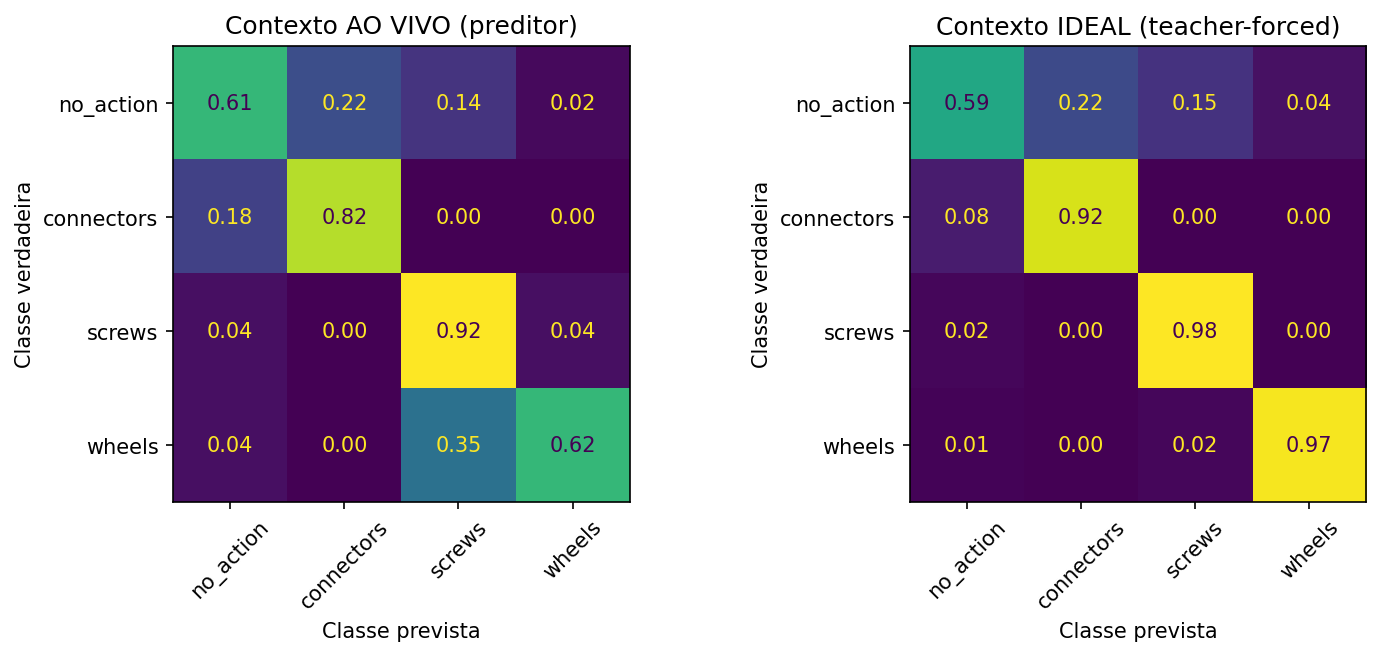
\includegraphics[width=\textwidth]{figures/cm_test.png}
\caption{Matrizes de confusão do teste (S02+S05), V2(10D), normalizadas por
linha (cada linha soma 1,0), no padrão do \texttt{hrc-finetune}. Esquerda:
contexto construído ao vivo pelo preditor. Direita: contexto ideal
(\emph{teacher-forced}). A diferença mais visível é a linha \texttt{wheels}:
com contexto ideal o \emph{recall} é 0,97; ao vivo cai para 0,62, com 0,35 da
massa vazando para \texttt{screws}.}
\label{fig:cm_test}
\end{figure}

O custo agregado de construir o contexto ao vivo é pequeno: \textbf{top-1 de
$70{,}9\%$ para $68{,}5\%$} ($-2{,}4$ p.p.). Mas a leitura por classe é mais
informativa e revela onde o preço é pago:

\begin{itemize}
  \item \texttt{get\_screws} e \texttt{get\_connectors} caem pouco (98,4\%$\to$92,4\%
    e 92,3\%$\to$82,0\%): o contexto ao vivo os sustenta bem.
  \item \texttt{get\_wheels} \textbf{despenca} (97,2\%$\to$61,7\%). A
    Figura~\ref{fig:cm_test} mostra que 0,35 dos quadros \texttt{wheels} são
    previstos como \texttt{screws}: as rodas vêm no fim da montagem, quando o
    contexto ao vivo já acumulou a maior deriva (Seção~\ref{sec:escala}), e o
    modelo confunde a fase final de parafusar com a de rodas.
  \item \texttt{no\_action} sobe ligeiramente (59,1\%$\to$61,4\%): parte dos
    erros de ação vira \texttt{no\_action}, a classe majoritária -- o mesmo
    efeito de mascaramento discutido nos relatórios anteriores, que é por que a
    diferença de top-1 ($-2{,}4$) subestima a degradação real por classe.
\end{itemize}

\subsection{Escalabilidade}
\label{sec:escala}

\paragraph{Generalização.} O top-1 ao vivo é $68{,}5\%$ no teste (não visto)
contra $73{,}7\%$ no treino -- uma diferença de $5{,}2$ p.p., compatível com a
lacuna de generalização já esperada para novos participantes/roteiros com poucos
dados (8 sessões, 2 participantes).

\paragraph{Estabilidade temporal.} A Tabela~\ref{tab:temporal} divide cada sessão
em três terços iguais e mede a acurácia ao vivo em cada um. A queda ao longo da
sessão é a assinatura da \emph{deriva} do contexto: como o vetor é cumulativo, os
pequenos erros de contagem se acumulam e o contexto do fim da sessão é o mais
distante do ideal.

\begin{table}[h]
\centering
\caption{Acurácia \emph{streaming} ao vivo por terço da sessão (início / meio /
fim), V2(10D), \texttt{send\_window}$=8$.}
\label{tab:temporal}
\begin{tabular}{lrrr}
\toprule
\emph{Split} & Início & Meio & Fim \\
\midrule
Teste  & 72,1\% & 70,1\% & 63,3\% \\
Treino & 75,2\% & 74,0\% & 72,0\% \\
\bottomrule
\end{tabular}
\end{table}

No teste a acurácia cai $8{,}8$ p.p.\ do primeiro ao último terço. É uma deriva
real, porém contida (bem menor que os $\sim$26 p.p.\ observados numa versão
preliminar com \texttt{send\_window}$=3$). A conclusão de escalabilidade:
\textbf{para janelas curtas o contexto ao vivo é confiável; para uso contínuo e
sessões longas, a deriva recomenda re-sincronizar o estado por eventos externos}
(Seção~\ref{sec:discussao}).

\subsection{Onde o contexto erra, e o papel do comando de voz}
\label{sec:onde-erra}

A Tabela~\ref{tab:dim} mostra o erro médio, dimensão a dimensão, entre o vetor de
contexto ao vivo e o ideal (no teste, sobre os quadros com predição). Ela
localiza a deriva: as dimensões que dependem da \emph{inferência da visão}
(estágio ativo, contagem de parafusos) derrapam mais, enquanto as controladas
pelo evento externo de voz (estágio \emph{four\_tubes} e seus parafusos) ficam
quase perfeitas.

\begin{table}[h]
\centering
\caption{Erro médio $|$ao vivo $-$ ideal$|$ por dimensão do contexto 10D (teste).
Dimensões ordenadas do maior para o menor erro.}
\label{tab:dim}
\begin{tabular}{lr}
\toprule
Dimensão do contexto & Erro médio \\
\midrule
\texttt{stage:none}          & 0,301 \\
\texttt{stage:top}           & 0,246 \\
\texttt{screws\_top / 4}     & 0,154 \\
\texttt{long tubes / 4}      & 0,153 \\
\texttt{screws\_bottom / 4}  & 0,112 \\
\texttt{short tubes / 8}     & 0,069 \\
\texttt{wheels / 4}          & 0,066 \\
\texttt{stage:bottom}        & 0,061 \\
\texttt{screws\_four\_tubes / 4} & 0,007 \\
\texttt{stage:four\_tubes}   & 0,000 \\
\bottomrule
\end{tabular}
\end{table}

\paragraph{Ablação do comando de voz.} Para testar diretamente a hipótese de que
o comando de voz importa para a contagem de tubos, rodamos a malha \emph{sem} o
evento \texttt{begin\_four\_tubes} (visão pura). O resultado confirma a hipótese:
sem o evento, o erro do contexto nas dimensões de tubo do estágio
\emph{four\_tubes} salta -- \texttt{short tubes} de $0{,}07$ para $0{,}30$ e
\texttt{screws\_four\_tubes} de $0{,}01$ para $0{,}42$ --, porque a voz é a única
fonte dos quatro tubos curtos daquele estágio. Em top-1 o efeito é menor mas
favorável ao evento ($68{,}5\%$ com voz vs.\ $66{,}5\%$ sem), coerente com a
Tabela~\ref{tab:dim}: como as dimensões controladas pela voz ficam corretas, o
evento ajuda tanto a fidelidade do estado quanto, marginalmente, a predição.
\textbf{O comando de voz (ou um gatilho externo equivalente) é, portanto,
necessário para a parte do contexto que a visão não consegue inferir sozinha.}

\subsection{Integridade das confirmações por sessão}
\label{sec:integridade}

A Tabela~\ref{tab:sessao} detalha, por sessão, quão bem a construção ao vivo
recupera o plano. Sete das oito sessões recuperam $\ge 0{,}83$ da sequência real,
com zero erros de transição; a exceção é \texttt{S08}, onde um segmento de
alcance rotulado \texttt{ignore} (não relacionado à entrega de tubos) é pulado e
a malha perde o fio -- um lembrete de que o rótulo \texttt{ignore} é usado para
finalidades distintas e nem todo bloco \texttt{ignore} é ``fora de tarefa''.
Note também que em \texttt{S03} e \texttt{S04} a acurácia ao vivo \emph{supera} a
do contexto ideal: nessas sessões curtas o contexto construído acompanha o plano
tão bem quanto o gabarito, e a variância de \emph{streaming} favorece o ao vivo.

\begin{table}[h]
\centering
\caption{Por sessão (V2(10D), \texttt{send\_window}$=8$): top-1 ao vivo vs.\
ideal, recuperação da sequência (LCS), erros de \texttt{PlanGraph} e
confirmações do modelo por classe. As duas sessões de teste em destaque.}
\label{tab:sessao}
\begin{tabular}{lrrrrr}
\toprule
Sessão & Top-1 ao vivo & Top-1 ideal & Seq. (LCS) & Erros plano & Confirm.\ (C/S/W) \\
\midrule
S01           & 66,5\% & 72,4\% & 0,96 & 0 & 8/12/5 \\
\textbf{S02}  & 58,3\% & 70,6\% & 0,83 & 0 & 8/14/1 \\
S03           & 80,1\% & 70,0\% & 1,00 & 0 & 5/4/0 \\
S04           & 82,1\% & 75,0\% & 1,00 & 0 & 6/9/0 \\
\textbf{S05}  & 75,6\% & 71,2\% & 0,92 & 0 & 13/10/5 \\
S06           & 73,6\% & 72,4\% & 0,96 & 0 & 9/11/6 \\
S07           & 77,3\% & 86,8\% & 0,67 & 1 & 8/9/0 \\
S08           & 67,5\% & 81,2\% & 0,24 & 0 & 4/2/0 \\
\bottomrule
\end{tabular}
\end{table}

A Tabela~\ref{tab:confconf} agrega, no teste, o que o modelo \emph{confirmou}
contra o que a pessoa de fato fazia no quadro da confirmação. Ela é a informação
mais acionável para o próximo ciclo de treino: fora da diagonal (e a linha
\texttt{no\_action}) estão as confirmações erradas que o treino precisa
desambiguar.

\begin{table}[h]
\centering
\caption{Confusão de confirmações no teste: linha = rótulo real no quadro da
confirmação; coluna = intenção confirmada pelo modelo. V2(10D),
\texttt{send\_window}$=8$.}
\label{tab:confconf}
\begin{tabular}{lrrrr}
\toprule
real $\backslash$ confirmado & no\_action & connectors & screws & wheels \\
\midrule
no\_action     & 0 & 11 & 2  & 0 \\
get\_connectors & 0 & 10 & 0  & 0 \\
get\_screws     & 0 & 0  & 19 & 1 \\
get\_wheels     & 0 & 0  & 3  & 5 \\
\bottomrule
\end{tabular}
\end{table}

Dois padrões se destacam: (i) \textbf{treze confirmações espúrias durante o
repouso} (linha \texttt{no\_action}: 11 como \texttt{connectors}, 2 como
\texttt{screws}) -- o modelo dispara intenção com a pessoa parada; e (ii)
\textbf{confusão \texttt{wheels}$\to$\texttt{screws}} (linha \texttt{get\_wheels}:
3 de 8 confirmadas como \texttt{screws}), coerente com o colapso do \emph{recall}
de rodas na Figura~\ref{fig:cm_test}.

\section{Discussão e recomendações}
\label{sec:discussao}

A construção ao vivo do contexto \emph{funciona} com os ajustes desta análise: o
custo em top-1 é de apenas $2{,}4$ p.p.\ no teste, a sequência do plano é
recuperada em $\ge 0{,}83$ na maioria das sessões e os erros de transição do
\texttt{PlanGraph} são zero no teste. As fragilidades que restam são concretas e
sugerem intervenções específicas, em ordem de impacto medido:

\begin{enumerate}
  \item \textbf{Confirmações espúrias no repouso são o erro nº 1}
    (Tabela~\ref{tab:confconf}). Um portão de movimento/confiança antes de
    confirmar e, sobretudo, \emph{exemplos negativos difíceis} de
    \texttt{no\_action} no treino atacariam a causa. Foi por isso que aumentar
    \texttt{send\_window} (que filtra picos isolados) teve o maior impacto isolado
    (Tabela~\ref{tab:sweep}).
  \item \textbf{Deriva temporal $\Rightarrow$ re-sincronização externa.} A queda
    de acurácia no fim da sessão (Tabela~\ref{tab:temporal}) vem do acúmulo de
    erro no contexto cumulativo. Re-sincronizar o estado por eventos externos
    confiáveis (o robô sabe o que entregou; a voz sinaliza mudanças de estágio),
    em vez de deduzir todo o estado só da visão, limita essa deriva. A ablação da
    Seção~\ref{sec:onde-erra} mostra que os eventos externos já disponíveis
    (\texttt{begin\_four\_tubes}) mantêm as dimensões que controlam praticamente
    sem erro.
  \item \textbf{A classe \texttt{get\_wheels} precisa de reforço.} Seu
    \emph{recall} ao vivo (62\%) é o mais frágil, por confusão com
    \texttt{get\_screws} na fase final (Figura~\ref{fig:cm_test},
    Tabela~\ref{tab:confconf}). Mais dados de rodas e/ou realce do contexto de
    estágio final no treino ajudariam a separá-las.
\end{enumerate}

Vale registrar que a exclusão dos trechos \texttt{ignore}
(Seção~\ref{sec:ignore}) foi importante para a limpeza da análise: numa versão
preliminar, as confirmações disparadas durante a entrega manual de tubos eram a
maior fonte de erros de transição do \texttt{PlanGraph}. Ao mesmo tempo,
\texttt{S08} mostra que o rótulo \texttt{ignore} cobre situações heterogêneas;
uma revisão da anotação (separar ``\emph{setup}/entrega manual'' de ``alcance
não pontuado'') tornaria tanto o treino quanto esta avaliação mais precisos.

\section{Conclusão}
\label{sec:conclusao}

O modelo treinado \emph{offline} sustenta-se em malha fechada: com o comando de
voz reproduzido pelo evento gravado e a janela de confirmação ajustada de 3 para
8, o contexto construído ao vivo pelo próprio preditor custa apenas $2{,}4$ p.p.\
de top-1 no teste em relação ao contexto ideal, com recuperação da sequência do
plano de $\ge 0{,}83$ na maioria das sessões e zero erros de transição do
\texttt{PlanGraph} no teste. A escalabilidade tem duas ressalvas mensuráveis: uma
deriva temporal (a acurácia cai ao longo da sessão, à medida que o contexto
cumulativo acumula erro) e a fragilidade da classe \texttt{get\_wheels} (confusão
com \texttt{get\_screws} na fase final). As três recomendações -- endurecer a
confirmação contra o repouso (com \emph{hard negatives} de \texttt{no\_action}),
re-sincronizar o estado por eventos externos confiáveis, e reforçar a classe de
rodas -- endereçam diretamente os erros medidos, e todas são compatíveis com a
infraestrutura já existente do projeto.

\begin{thebibliography}{9}
\bibitem{yu2025}
P. Yu, A. Abuduweili, R. Liu, C. Liu.
\emph{Robustifying Long-term Human-Robot Collaboration through a
Multimodal and Hierarchical Framework}.
arXiv:2411.15711, 2025.
\end{thebibliography}

\end{document}
